\documentclass[tikz]{standalone}
\usepackage{tikz}
\usepackage{color}
\usepackage[utf8]{inputenc}
\usetikzlibrary{shapes, positioning}
\definecolor{aliceblue}{rgb}{0.94, 0.97, 1.0}
\definecolor{aqua}{rgb}{0.0, 1.0, 1.0}
\begin{document}
	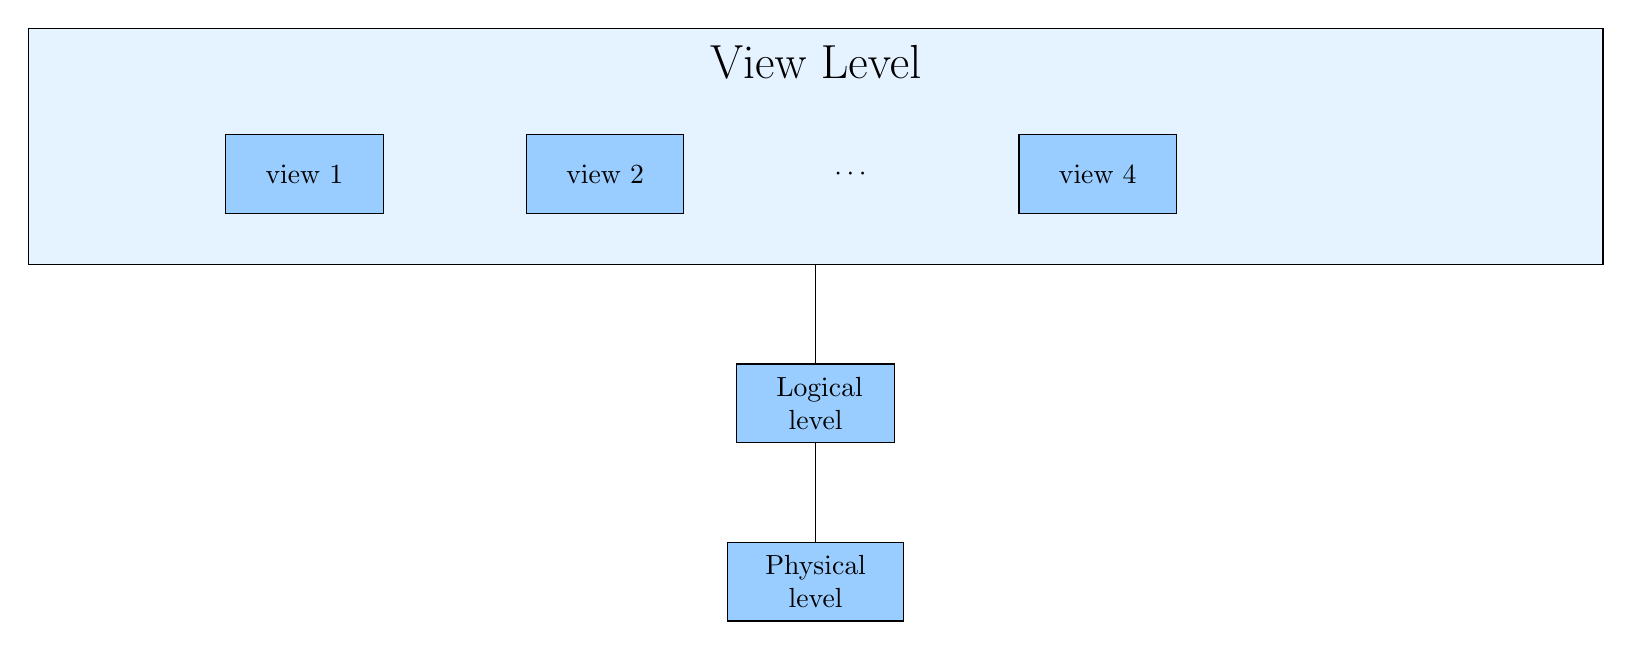
\begin{tikzpicture}
	\node[draw, rectangle,fill=aqua!50!blue!10
	, text width=4cm,minimum height=3cm,minimum width=20cm, align=center, label={[anchor=north, inner sep=0pt, yshift=-0.6em, text=black]north:\LARGE{View Level}}] at 
	(0,0) (rect) {};
	
	\node[draw, rectangle,fill=aqua!50!blue!40
	, text width=1cm,minimum height=1cm,minimum width=2cm, align=center] at 
	([xshift=10em, yshift=-1em]rect.west) (v1) {view 1};
	\node[draw, rectangle,fill=aqua!50!blue!40
	, text width=1cm,minimum height=1cm,minimum width=2cm, align=center] at 
	([xshift=8em]v1.east) (v2) {view 2};
	\node[draw=none, align=center] at 
	([xshift=6em]v2.east) (v3) {$\cdots$};
	\node[draw, rectangle,fill=aqua!50!blue!40
	, text width=1cm,minimum height=1cm,minimum width=2cm, align=center] at 
	([xshift=8em]v3.east) (v4) {view 4};
	
	\node[draw, rectangle,fill=aqua!50!blue!40
	, text width=1cm,minimum height=1cm,minimum width=2cm, align=center] at 
	([yshift=-5em]rect.south) (ll) {Logical level};
	\node[draw, rectangle,fill=aqua!50!blue!40
	, text width=2cm,minimum height=1cm,minimum width=2cm, align=center] at 
	([yshift=-5em]ll.south) (pl) {Physical level};
	
	\draw (rect) -- (ll);
	\draw (ll) -- (pl);
	\end{tikzpicture}
	
\end{document}
